% !Mode:: "TeX:UTF-8"

\documentclass[a4paper,11pt,onecolumn,twoside]{article}
\usepackage{fancyhdr}
\usepackage{amsmath,amsfonts,amssymb,amsthm}
\usepackage{graphicx}
\usepackage{verbatim}
\usepackage{mathptmx}
\usepackage{booktabs}
\usepackage[labelfont=bf]{caption}
\usepackage{indentfirst}
\usepackage{caption}
\usepackage{setspace}
\usepackage{enumitem}
\usepackage{subfigure}
\usepackage{fontspec}
\usepackage{appendix}
\usepackage{listings}
\usepackage{xeCJK}
\newtheorem{lemma}{引理}[section]% Please change the following fonts if they are not available.
\setmainfont{Times New Roman}

\addtolength{\topmargin}{-54pt}
\setlength{\oddsidemargin}{-0.9cm}
\setlength{\evensidemargin}{\oddsidemargin}
\setlength{\textwidth}{17.00cm}
\setlength{\textheight}{24.50cm}

\renewcommand{\baselinestretch}{1.1}
\parindent 22pt

\title{\textbf{第六次上机实验报告}}
\author{
马宇恒
\\[2pt]
{\small \textit{匡亚明学院 171240510}}}
\date{}
\fancypagestyle{firststyle}
{
   \fancyhf{}
   \fancyhead[C]{数值计算实验报告}
   \fancyhead[R]{\thepage}
}

\pagestyle{fancy}
\fancyhf{}

\fancyhead[LE,RO]{\thepage}
\fancyhead[CE]{数值计算与实验}
\fancyhead[RE]{}
\fancyhead[CO]{}
\fancyhead[LO]{}

\setlist{nolistsep}
\captionsetup{font=small}

\newcommand{\supercite}[1]{\textsuperscript{\cite{#1}}}
\begin{document}
\maketitle
\thispagestyle{firststyle}
\setlength{\oddsidemargin}{ 1cm}
\setlength{\evensidemargin}{\oddsidemargin}
\setlength{\textwidth}{15.50cm}
\vspace{-.8cm}


\setcounter{page}{1}

\setlength{\oddsidemargin}{-.5cm}  % 3.17cm - 1 inch
\setlength{\evensidemargin}{\oddsidemargin}
\setlength{\textwidth}{17.00cm}

\section{实验目的}
利用下列条件做插值逼近,并与$$\frac{1}{1+x^2}$$的图像比较。
\begin{itemize}
\item 用等距节点 $x _ { i } = - 5 + i , \quad i = 0,1 , \cdots , 10$给出它的10次Newton插值多项式的图像。
\item 用节点$x _ { i } = 5 \cos \left( \frac { 2 i + 1 } { 42 } \pi \right) , i = 0,1 , \cdots , 20$ 给出它的20次Lagrange插值多项式的图像。
\item 用等距节点$x _ { i } = - 5 + i , \quad i = 0,1 , \cdots , 10$给出它的分段线性插值函数的图像。
\item 用等距节点$x _ { i } = - 5 + i , \quad i = 0,1 , \cdots , 10$给出它的三次自然样条插值函数的图像。
\item 用等距节点$x _ { i } = - 5 + i , \quad i = 0,1 , \cdots , 10$给出它的分段三次Hermite插值函数的图像。

\end{itemize}

\section{任务一}
写成默认参数的函数形式,输入x值,输出插值函数的值。
\subsection{程序}
\begin{lstlisting}
function result =newton(x,c)
if nargin<2
    c=-5:5;
end
n=length(c)-1;
dq=zeros(n+1);
for i =1:n+1
    dq(i,1)=f(c(i));
end
for j = 2:n+1
    for i= j:n+1
        dq(i,j)=(dq(i,j-1)-dq(i-1,j-1))/(c(i)-c(i-j+1));
    end
end
p=zeros(1,n+1);
p(1,n+1)=dq(1,1);
for i = 2:n+1
    p=p+[zeros(1,n+1-i),dq(i,i)*poly(c(1:i-1))];
end
result=p(1);
for i =2:n+1
    result=result*x+p(i);
end
end
\end{lstlisting}
\subsection{结果与分析}
\begin{figure}[htbp]
  \centering
  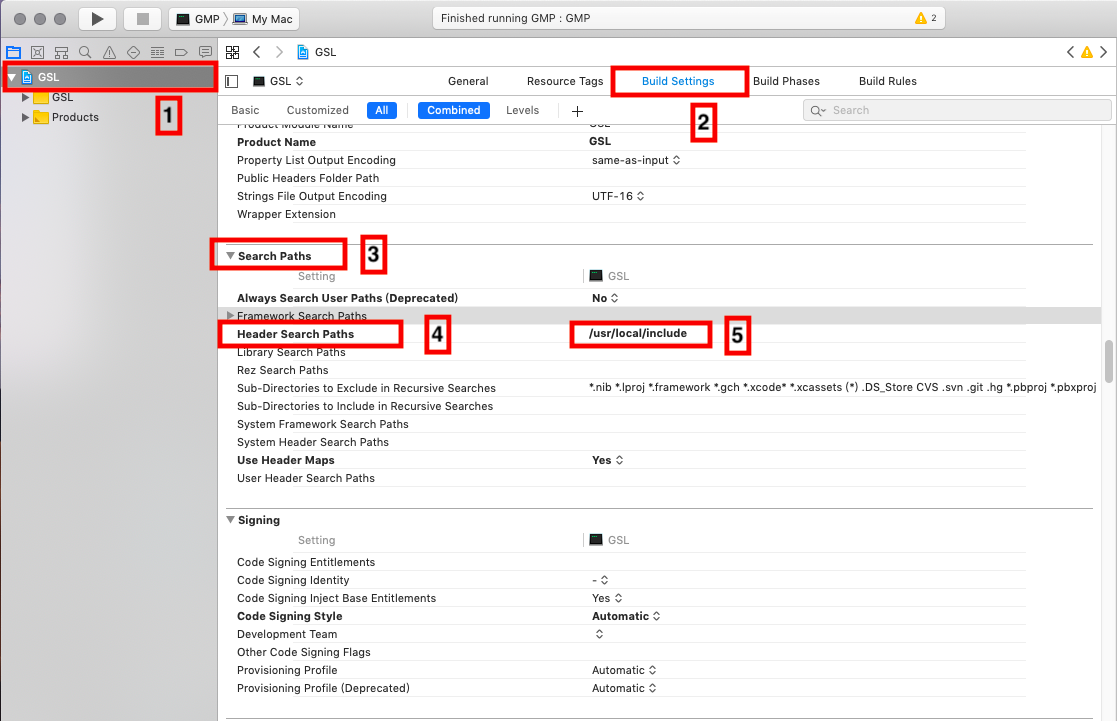
\includegraphics[width=0.6\textwidth]{1.png}
  \caption{牛顿插值} \label{1}
\end{figure}
Runge效应比较明显。接下来我们使用拉格朗日插值,但是改变插值点以减弱Runge效应。

\section{任务二}
写成默认参数的函数形式,输入x值,输出插值函数的值。
\subsection{程序}
\begin{lstlisting}
function result =lagrange(x,c)
if nargin<2
    c=0:20;
    c=5*cos(pi*(2*c+1)/42);
end
n=length(c)-1;
p=zeros(1,n+1);
for i = 1:n+1
    temp=c;
    temp(i)=[];
    p=p+f(c(i))*poly(temp)/prod(c(i)*ones(1,n)-temp);
end
result=p(1);
for i =2:n+1
    result=result*x+p(i);
end
end
\end{lstlisting}
\subsection{结果与分析}
\begin{figure}[htbp]
  \centering
  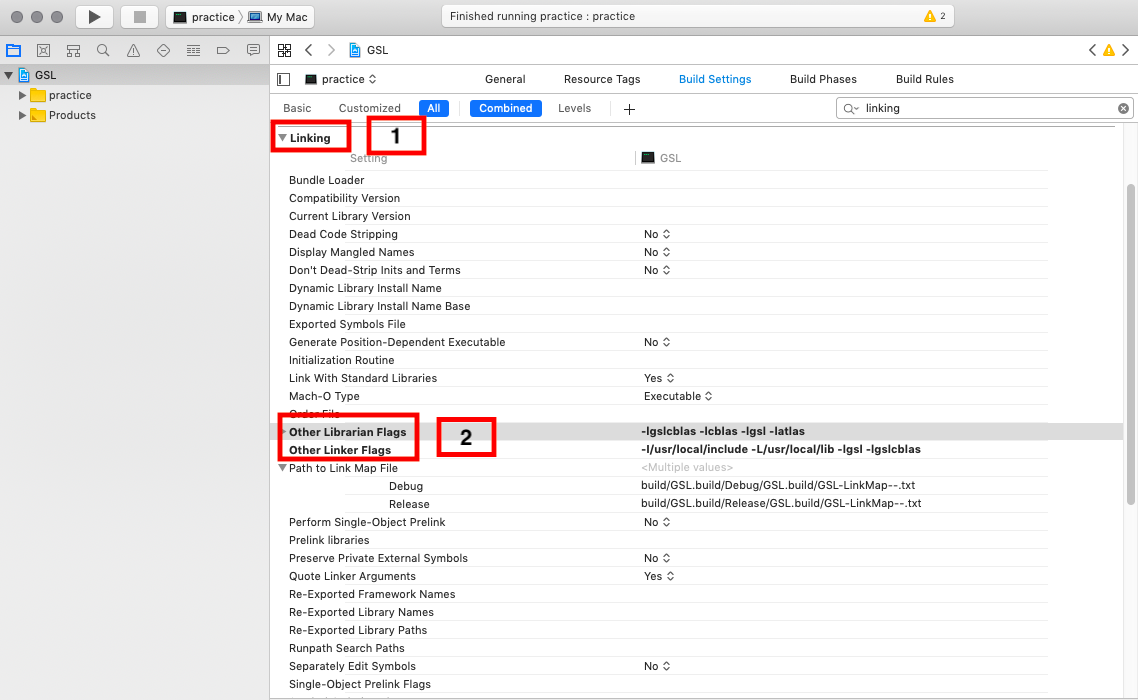
\includegraphics[width=0.6\textwidth]{2.png}
  \caption{拉格朗日插值} \label{2}
\end{figure}
拟合效果相比前者理想很多。不过仍能够看到Runge的出现。于是我们使用分段插值来彻底消除Runge。

\section{任务三}
写成默认参数的函数形式,输入x值,输出插值函数的值。
\subsection{程序}
\begin{lstlisting}
function result= line(x,c)
if nargin<2
    c=-5:5;
end
c=sort(c);
index=find(sort([c,x])==x);
index=index(1)-1;
result= (f(c(index+1))-f(c(index)))/(c(index+1)-c(index))*(x-c(index))+f(c(index));
end
\end{lstlisting}
\subsection{结果与分析}
\begin{figure}[htbp]
  \centering
  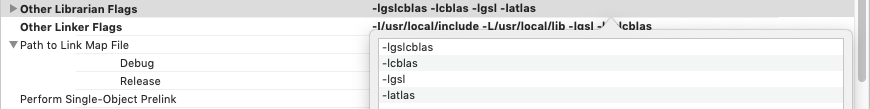
\includegraphics[width=0.6\textwidth]{3.png}
  \caption{分段线性插值} \label{3}
\end{figure}
线性插值略显僵硬,不过可以看到效果对于导数不太大的部分尚可,Runge也基本消失。前三种方法或在边界处想过不好,或在中心处效果不好。

\section{任务四}
写成默认参数的函数形式,输入x值,输出插值函数的值。
\subsection{程序一}
\begin{lstlisting}
function result = natural(x,c)
if nargin<2
    c=-5:5;
end
n=length(c)-1;
c=sort(c);
index=find(sort([c,x])==x);
index=index(1)-1;
d=zeros(1,n);
h=zeros(1,n);
m=zeros(1,n-1);
for i =1:n
    h(i)=c(i+1)-c(i);
end
for i=2:n
    d(i)=(f(c(i+1))-f(c(i)))/h(i)-(f(c(i))-f(c(i-1)))/h(i-1);
end
d(1)=[];
H=zeros(n-1);
H(1,1)=2*(h(1)+h(2));
for i=2:n-1
   H(i,i)=2*(h(i)+h(i+1));
   H(i,i-1)=h(i);
   H(i-1,i)=h(i);
end
t=zeros(1,n-1);
t(1)=gg(c(1))*h(1)/6;
t(n-1)=gg(c(n+1))*h(n)/6;
m=pursue(H,6*(d-t));
m=[gg(c(1)),m,gg(c(n+1))];
result=((c(index+1)-x)^3*m(index)/6+(x-c(index))^3*m(index+1)/6)/h(index)+f(c(index));
result=result+(x-c(index))*(f(c(index+1))-f(c(index)))/h(index);
result=result-h(index)*h(index)*(1/6)*(m(index)+(m(index+1)-m(index))*(x-c(index))/h(index));
end
\end{lstlisting}
\subsection{代码二(追赶法)}
\begin{lstlisting}
function result=pursue(a,b)
n=length(b);
a(1,2)=a(1,2)/a(1,1);
for i = 2:n-1
    a(i,i)=a(i,i)-a(i,i-1)*a(i-1,i);
    a(i,i+1)=a(i,i+1)/a(i,i);
end
a(n,n)=a(n,n)-a(n,n-1)*a(n-1,n);
b(1)=b(1)/a(1,1);
for i = 2:n
   b(i)=(b(i)-a(i,i-1)*b(i-1))/a(i,i); 
end
for i=1:n-1
   b(n-i)=b(n-i)-b(n-i+1)*a(n-i,n-i+1);
end
result=b;
end
\end{lstlisting}
\subsection{结果与分析}
\begin{figure}[htbp]
  \centering
  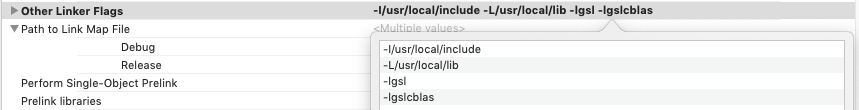
\includegraphics[width=0.6\textwidth]{4.png}
  \caption{三次自然样条插值} \label{4}
\end{figure}
可以看到效果相当的优秀,基本没什么好点评的。唯一缺点就是代码太长了。

\section{任务五}
写成默认参数的函数形式,输入x值,输出插值函数的值。
\subsection{程序}
\begin{lstlisting}
function result = hermite(x,c)
if nargin<2
    c=floor(x):(1/3):floor(x)+1;
end
n=length(c)-1;
p=zeros(1,2*n+2);
for i=1:n+1
    temp=c;
    temp(i)=[];
    l=poly(temp)/prod(c(i)-temp);
    ls=conv(l,l);
   p=p+f(c(i))* conv([0,1]-2*poly(c(i))*sum((c(i)-temp).^-1),ls);
end
for i=1:n+1
    temp=c;
    temp(i)=[];
    l=poly(temp)*prod((c(i)-temp).^-1);
    ls=conv(l,l);
    p=p+g(c(i))*conv(poly(c(i)),ls);
end
result=p(1);
for i =2:(2*n+2)
    result=result*x+p(i);
end
end
\end{lstlisting}
\subsection{结果与分析}
\newpage
\begin{figure}[htbp]
  \centering
  \includegraphics[width=0.6\textwidth]{5.png}
  \caption{分段埃尔米特插值} \label{5}
\end{figure}

两种颜色都合成一种了,这效果没谁了。而且代码也不是非常复杂。

\section{总结}
\begin{figure}[htbp]
  \centering
  \includegraphics[width=0.7\textwidth]{6.jpg}
 \caption{汇总绘图}\label{6}
\end{figure}
所有函数在一起绘图,可以看到效果逐渐变好的过程。

\end{document}
